\chapter{Распознавание по радужке с мобильного устройства}

\section{Основные трудности при распознавании человека по радужке}
\label{sec:main_difficulties_mobile}

Биометрические технологии распознавания хорошо зарекомендовали себя и заняли нишу в решении задач, связанных с обеспечением безопасности. Говоря о мобильных устройствах, существенное количество современных персональных устройств (смартфонов, планшетов и т.д.) оснащены компактными сканерами отпечатков пальцев, предназначенных для аутентификации пользователя. Не смотря на то, что методы аутентификации по отпечаткам пальцев демонстрируют достаточно высокую точность распознавания, они все еще имеют существенные недостатки~\cite{daugman_probing_2006}. Среди всех биометрических модальностей, рассматриваемых в качестве кандидатов для замены либо объединения с отпечатками, радужная оболочка глаза остается одной из самых привлекательных~\cite{bowyer_survey_2008,corcoran_2014,daugman_epigenetic_2001,survey_10-15}.

Регистрация изображения радужки обычно производится с использованием камеры высокого разрешения в ближнем инфракрасном (БИК), либо в видимом диапазоне длин волн~\cite{prabhakar_2011} в фиксированных, практически <<лабораторных>> условиях окружения. Требования, предъявляемые к системе и процессу регистрации изложены в стандарте ISO/IEC 19794-6:2011~\cite{iso_iris}. Когда речь заходит о массовом производстве, стоимость, компактность и удобство использования становятся существенными, и поэтому не все, упомянутые в стандарте~\cite{iso_iris}, требования могут быть удовлетворены. В значительной степени это касается системы регистрации изображения. Не менее важным моментом является то, что рынок мобильных устройств подразумевает их использование по всему миру, становится важно учитывать все возможные поведенческие и расовые особенности конечных пользователей. По этой причине, в частности, не допускается использование изображений, зарегистрированных в видимом диапазоне спектра, т.к. текстура радужки темных (в основном коричневых) оттенков оказывается практически неразличимой. Более подробно о преимуществах распознавания по радужке в БИК диапазоне изложено в работах~\cite{iso_iris,corcoran_2014,daugman_epigenetic_2001,daugman_how_works}, а проблемы, связанные с системами регистрации изображения радужки, подробно описаны в работах~\cite{prabhakar_2011,corcoran_2014}.

\begin{figure}[t!]
	\centering
	\includegraphics[width=0.95\columnwidth]{pictures/mobile-examples.png}
	\caption{Примеры изображений полученных при фиксированных условиях окружения (сверху), и изображений, полученных при помощи мобильного устройства (снизу)}
	\label{fig:casia-mobile-examples}
\end{figure}

Использование мобильного устройства в качестве биометрического сенсора подразумевает его способность обрабатывать биометрические данные при постоянном изменении окружения и учитывать поведение пользователя. Места использования устройства могут сильно различаться по уровням освещенности (от $10^{-4}$ до более $10^5$ люкс под прямыми солнечными лучами), спектрам излучения источников, спектру поглощения и отражения окружающих объектов и многим другим параметрам. С другой стороны, следует учитывать и особенности пользователя: он может носить очки, контактные линзы; может произвести попытку аутентификации при ходьбе или страдать от тремора рук, тем самым вызывая дрожание устройства; пользователь может удерживать устройство слишком далеко или близко к лицу, так, что радужка оказывается вне диапазона глубины резкости камеры, и её изображение получается размытым; зрачки пользователя могут быть сильно расширены или сужены в зависимости от уровня освещенности и по другим причинам~\cite{matveev_doctor_thesis,thavalengal_2016,odinokikh_hprec_2018}; область радужки может быть сильно затенена веками и ресницами, если глаз пользователя недостаточно открыт. Все упомянутые факторы влияют на качество входных биометрических данных (Рис.~\ref{fig:casia-mobile-examples}) и, как следствие, на точность распознавания~\cite{tabassi_2011}.

В дополнение ко всем вышеперечисленным факторам, мобильная система должна быть простой и удобной в использовании. Для биометрической системы удобство определяется простотой взаимодействия с пользователем и высокой скоростью распознавания, где последняя обусловлена вычислительной сложностью применяемого метода (Рис.~\ref{fig:iris_mobile_problems}). Между сложностью и энергопотреблением существует компромисс, который важно учитывать при разработке мобильных алгоритмов. Процесс аутентификации должен осуществляться с частотой поступления кадров и, в то же время, потреблять минимальное количество энергии устройства.

При разработке мобильных биометрических систем также следует принимать во внимание важное требование, предъявляемое к системам с высоким уровнем защиты. а именно, полное отсутствие доступа извне к данным, которые они обрабатывают. К таким данным относятся пин-коды, иная персональная информация и, особенно, биометрические данные. На сегодняшний день существует технологии, предоставляющие возможность обеспечить достаточный уровень защищенности данных. Они все представляют систему на чипе (SoC, System on Chip), являющуюся защищенной частью центрального процессора устройства, с развернутой на нем отдельной операционной системой, например TrustZone от ARM или Qualcomm~\cite{arm}. Такого рода системы накладывают дополнительные ограничения на приложения, с которыми они работают. Ограничения выражаются в виде еще более заниженной доступной тактовой частоте процессора, невозможности использовать многопоточность и существенно ограниченном обьеме доступной оперативной памяти.

\section{Метод аутентификации по радужке c мобильного устройства}
\label{sec:auth_method}

Несмотря на успешное внедрение множества биометрических систем распознавания по радужке по всему миру, мобильные приложения этой технологии являются новой областью для исследований~\cite{btas_competition_2016,brief_survey_2014}. Это связано с тем, что известные на сегодняшний день алгоритмы и решения не способны обеспечить достаточную точность распознавания на данных, полученных с мобильного устройства. В большинстве исследований в данной области используются изображения, полученные в видимом диапазоне\cite{barra_2015,demarsico_2014,raja_2015}. В работе Thavalengal и др.~\cite{thavalengal_2015} исследована возможность использования комбинированного решения, использующего изображения радужки, полученные одновременно в видимом и БИК диапазонах. Утверждается, что для предложенной системы и метода, распознавание на расстоянии превышающем 15 см все еще затруднено. Примером решения, использующего БИК диапазон, является работа Zhang и др.~\cite{zhang_2015}, в которой представлены результаты, демонстрирующие перспективность подхода с объединением для распознавания двух модальностей: радужки и лица. Апробация метода производилась на внутренней базе данных радужек и лиц. Одной из наиболее релевантных работ, предлагающих использование БИК диапазона для мобильных приложений, является~\cite{jeong_2005}. Предлагается использовать дополнительные факторы, оказывающие влияние на качество изображения радужки, в частности, уровни освещенности и смазанности при оценке качества изображения и сравнении биометрических эталонов.

На сегодняшний день уже существует несколько коммерческих решений для распознавания человека по радужке с мобильного устройства. Первый смартфон с технологией распознавания по радужной оболочке глаза Delta ID Inc.~\cite{deltaId,deltaId_ref} был представлен компанией Fujitsu в 2015 году~\cite{fujitsu}. В 2016 году компания Microsoft представила серию смартфонов Lumia 950~\cite{lumia_950}, оснащённых сканером радужки. Следом еще несколько компаний представили свои решения. Упомянутые компании использовали собственные данные, собранные для исследований и тестирования своих решений. Результаты по производительности алгоритмов не были опубликованы.

В данной главе представлено алгоритмическое решение для аутентификации человека по радужке, способное обеспечить точность и скорость распознавания достаточные для применения в мобильных приложениях. Основными особенностями метода являются: многостадийная структура алгоритма; новый подход к оценке качества изображения, позволяющий дать исчерпывающую оценку изображению радужки с учетом особенностей работы с мобильным устройством; а также новый адаптивный метод квантования вектора признаков радужной оболочки глаза. Данные особенности позволяют осуществлять распознавание в режиме реального времени в условиях сильного изменения окружения и обеспечить обратную связь с пользователем устройства. Решение детально описано в~\cite{odinokikh_hprec_2018}.

\subsection{Структура алгоритма распознавания}
\label{subsec:algorithm_structure}

Основная идея предлагаемой структуры алгоритма состоит в том, чтобы выполнять наиболее вычислительно сложные операции только с изображениями самого высокого качества. В данном случае под качеством понимается совокупность критериев, отражающих пригодность изображения радужки для извлечения особенностей и распознавания. Весь алгоритмический конвейер можно разделить на несколько частей, объединенных промежуточными этапами выбора изображений наилучшего качества. Общая схема предложенного алгоритма распознавания по радужной оболочке глаза с мобильного устройства представлена на Рис.~\ref{fig:algorithm_structure}.

\begin{figure}[!h]
	\centering
	\includegraphics[width=0.85\columnwidth]{pictures/algorithm_structure.png}
	\caption{Блок схема алгоритма распознавания по радужной оболочке глаза с мобильного устройства}
	\label{fig:algorithm_structure}
\end{figure}

На приведенной схеме (Рис.~\ref{fig:algorithm_structure}), можно выделить два основных блока обработки (до буфера изображений и после). Операции первого блока начинаются с получения изображения и заканчиваются вычислением промежуточного показателя качества $QM$ и помещении изображения в буфер. Операции второго блока начинаются с выбора из буфера изображения, для которого текущее значение $QM$ является максимальным среди всех, находящихся в буфере, а заканчивается выделением уникальных особенностей и построением вектора признаков радужки.

Первый блок осуществляет обработку данных с частотой поступления кадров. На первом этапе производится выделение области глаза на входном изображении. Предложенный метод основан на применении метода MLBP, предложенного в работе~\cite{kaushik_lbp_2014}, продемонстрировавшим наилучшие результаты для изображений c мобильного устройства. Полученные изображения проходят процедуру предобработки, включающую в себя подавление шума, а также повышения контрастности на границах зрачка и радужки. Предобработка производится с использованием оператора Шарра, представляющего из себя модификацию фильтра Собела, обладающую свойством более высокой вращательной симметрии~\cite{scharr_2007}. Фильтрация производится путем свертки входного изображения с заранее подобранным набором ядер Шарра. Далее на изображении производится выделение зрачка, путем определения координат его центра и границы. различные подходы к выделению зрачка рассмотрены в~\cite{matveev_doctor_thesis}. Для простоты в предложенном методе зрачок параметрически представляется в виде окружности, имеющей центр $(x_p,y_p)$ и радиус $r_p$. Зрачок также часто описывают эллипсом либо фигурой сложной формы. Выделение зрачка, также, обычно производится в несколько этапов. В большинстве работ, с целью ускорения вычислений, обычно можно выделить два основных этапа: грубая оценка параметров и их последующее уточнение. Методы грубой оценки зависят от условий применения. Здесь для грубой оценки предлагается метод, основанный на применении сверточных нейронных сетей, подробно описанный в главе~\ref{sec:segm_method}, а для уточнения используется интегро-дифференциальный оператор Догмана (\ref{eq:daugman_ido})~\cite{daugman_how_works}.

\begin{equation}\label{eq:daugman_ido}
\max \limits_{(r,x_0,y_0)} \left | G_\sigma (r) * 
{\frac{\partial}{\partial r} \oint \limits_{r, x_0, y_0} 
	{\frac{I(x,y)}{2 \pi r} ds}} \right |,
\end{equation}

\noindent
где $I(x, y)$ — яркость изображения.

\noindent
Оператор осуществляет поиск области на изображении, где достигается максимум частной производной от нормализованного интеграла по $r$ по направлению увеличения величины радиуса. Несколько модификаций подхода Догмана рассмотрены в работах~\cite{alonso_12,hu_11,jeong_10,mahadeo_12}. Далее производится оценка положения век на изображении. Их положение описывается координатами точек $E_u$ и $E_l$ для верхнего и нижнего век соответственно, как показано на рис.~\ref{fig:eyelid_position}. Предложенный метод определения положения век подробно описан в работе~\cite{odinokikh_eyelids_2016} и основан на применении набора разнонаправленных фильтров Габора для предобработки, и последующим уточнением границы века модификацией интегро-дифференциального оператора для параболический кривой (\ref{eq:daugman_ido_parabolic}).

\begin{equation}\label{eq:daugman_ido_parabolic}
\max \limits_{(a,k,h)} \left |\sum_{a}\sum_{k} G_\sigma * 
{\frac{\partial}{\partial h} \sum_{a} (y-k)^2-4a(x-h)} \right |,
\end{equation}

\noindent
где $(k, h)$ — вершина параболы, $a$ — её кривизна.

\begin{figure}[!h]
	\centering
	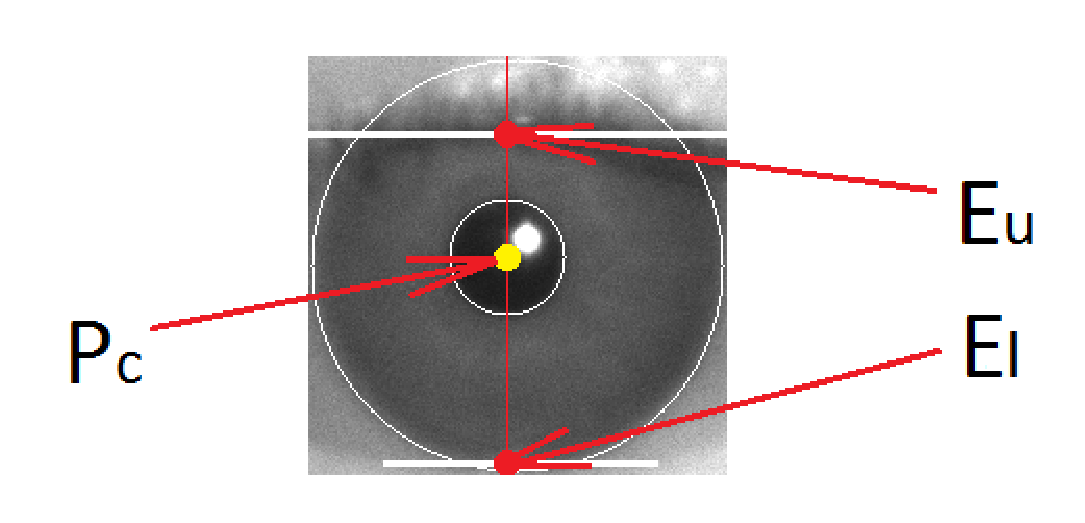
\includegraphics[width=0.5\columnwidth]{pictures/eyelid_position_pointers.eps}
	\caption{Определение положения верхнего $E_u$ и нижнего $E_l$ век, $P_c$ - центр зрачка}
	\label{fig:eyelid_position}
\end{figure}

\noindent
Вычисление промежуточного показателя качества является завершающей операцией первого блока и может производится различными способами. В данной работе в качестве оценки предлагается вычисление взвешенной суммы по нескольким накопленным в процессе обработки параметрам качества, среди которых: средние яркости полного кадра $I_{avg}^f$ и области глаза $I_{avg}^e$ (Рис.~\ref{fig:eyelid_position}), значение контраста на границе зрачок-радужка $C_{pi}$, степень открытости глаза $NEO$ (\ref{eq:neo_p}), выраженная по значениям $E_l$ и $E_u$ (Рис.~\ref{fig:eyelid_position}). Коэффициенты регрессии между набором используемых метрик и значением математического ожидания соответствующего распределения степени схожести для пар сравнений свой со своим предложено использовать в качестве весов для вычисления финального показателя качества.

Поскольку входные данные представляют собой видеопоследовательность, а не единичный кадр, можно выбирать изображения наилучшего качества в течение заранее определенного периода времени по завершению любого этапа алгоритма. Выбор может быть выполнен с использованием показателей качества, которые были оценены до помещения изображения в буфер (Рис.~\ref{fig:algorithm_structure}). После того как буфер полностью заполнен, каждый последующий кадр вытесняет один из кадров худшего качества в течение предопределенного времени. Как только заданное время истекло, выбранные изображения переносятся на второй этап обработки. В качестве временной константы может быть выбрано время полной обработки изображения на втором этапе.

Второй этап состоит из более вычислительно сложных операций. Обрабатываются только изображения из буфера. Этап начинается с поиска центра $(x_i,y_i)$ и радиуса $r_i$ радужки на изображении глаза с использованием информации о параметрах зрачка. Используемый подход к поиску аналогичен тому, что использовался для поиска зрачка. Информация о расположении век используется здесь для выбора диапазона углов при обходе контура интегро-дифференциальным оператором. Информация о положении век используется для определения области поиска интегро-дифференциальным оператором. Для удаления ресниц и частично затенений используется подход, описанный в~\cite{aligholizadeh_2011}. Далее над изображениями радужки полученной маски осуществляется операция нормализации (\ref{eq:certesian-polar}). Последним этапом второго блока является извлечение уникальных особенностей радужки и построение вектора признаков.

Извлечение особенностей радужки производится для каждого кадра, прошедшего все проверки по качеству. Заранее определенное количество векторов признаков, полученное в процессе регистрации ($N_E$) сохраняется в базе данных. Все они используются в дальнейшем для сравнения. Так как, возможность накапливать векторы признаков предлагается использовать и при верификации, существует несколько вариантов их использования. Метод сравнения <<каждый с каждым>> подразумевает $N_E \times N_V$ количество сравнений, а это не всегда оправдано ($N_V$ - текущее количество векторов признаков в режиме верификации). Для того чтобы уменьшить количество сравнений, несколько векторов признаков могут быть отобраны в качестве наиболее репрезентативных. Правило отбора таких векторов основано на измерении для них степени схожести внутри одного класса. Пара векторов, для которых степень схожести минимальна выбираются в качестве образцов для последующего сравнения с векторами, хранящимися в базе данных. Таким образом количество сравнений уменьшается и становится равным $0.5*N_V(N_V-1)+2N_E$. Если для $N_E$ и $N_V$ выполняется условие $N_E > N_V/2$, то количество сравнений значительно уменьшается.


\subsection{Оценка качества изображения радужки}
\label{subsec:quality_assessment}

Оценка качества изображения является неотъемлемым этапом распознавания~\cite{matveev_doctor_thesis}. В литературе известно множество подходов к оценке качества изображения радужки~\cite{czajka_2013,chen_2012,galbally_2012,feddaoui_2011}. Однако, большинство из них не рассматривает мобильные приложения.
Подход, описанный в данной работе, имеет несколько ключевых особенностей по сравнению с методами, известными ранее~\cite{hamza_patent_2012,prabhakar_patent_2013}.

Главной особенностью решения является предложенный набор критериев качества изображения радужки. Набор составлен из метрик, позволяющих оценивать качество с учетом большинства возможных сценариев использования устройства. Оценка по каждому из критериев производится сразу после того, как произведено соответствующее измерение.

Персональное мобильное устройство подразумевает постоянное взаимодействие с пользователем. По этой причине второй особенностью предложенного решения является способность осуществлять обратную связь с пользователем устройства. В случае отсеивания кадра по какому-либо критерию качества, пользователю автоматически выводится подсказка в понятной для него форме. Например, если вычисленное расстояние до лица выходит за заранее определенный допустимый предел, то пользователю будет предложено расположить устройство ближе либо дальше.

\begin{figure}[t!]
	\centering
	\includegraphics[width=0.95\columnwidth]{pictures/qa_structure.png}
	\caption{Общая схема алгоритма оценки качества изображения}
	\label{fig:qa_structure}
\end{figure}

Оценка качества также позволяет поддерживать обратную связь не только с пользователем, но и с аппаратной частью устройства, обеспечивая корректировку параметров системы регистрации изображения, с целью получения кадров наилучшего качества (подробнее в заявке на изобретение~\cite{gnatyuk_patent_2018}). Например, изображение области глаза было классифицировано как переэкспонированное. Алгоритм автоматически корректирует значение экспозиции для регистрации последующего кадра. На схеме (Рис.~\ref{fig:qa_structure}) изображена структура алгоритма оценки качества изображения. Обратная связь с пользователем и аппаратной частью условно обозначена буквой $F (feedback)$ со стрелкой.

\subsection{Использование дополнительных сенсоров}
\label{subsec:sensor_usage}

Отличительной особенностью метода является использование информации с дополнительных сенсоров, доступных для использования внутри устройства. Так, например, информация об уровне освещенности, данные с дальномера и иные доступные данные могут быть использованы для подстройки как параметров аппаратной части устройства, так и алгоритма. Таким образом реализуется связь между ключевыми компонентами биометрической системы: пользователем, аппаратной и программной частями устройства (Рис.~\ref{fig:hw_sw_user_scheme}). Детальное описание предложенного метода приведено в заявке~\cite{odinokikh_patent_2017_irec_ru}.

\begin{figure}[t!]
	\centering
	\includegraphics[width=0.95\columnwidth]{pictures/hw-sw-user-scheme.png}
	\caption{Условная схема взаимодействия между элементами системы распознавания}
	\label{fig:hw_sw_user_scheme}
\end{figure}

Вводятся дополнительные метрики оценки качества, позволяющие ускорить процесс обработки информации внутри алгоритма. Обе преложенные метрики (\ref{eq:neo_p}, \ref{eq:neo_i}) описывают уровень открытости глаза на различных этапах алгоритма с использованием информации о положении век $E_u$ и $E_l$.

\begin{equation}\label{eq:neo_p}
	NEO_p=\frac{|E_l-E_u|}{R_p}
\end{equation}

\begin{equation}\label{eq:neo_i}
	NEO_i=\frac{|E_l-E_u|}{R_i}
\end{equation}

\noindent
Метрики $NEO_p$ и $NEO_i$  (NEO, сокр. - normalized eye opening) вычисляются и используются на разных этапах алгоритма, сразу, как только информация о значения радиусов зрачка $R_p$ и радужки $R_i$ становится доступной. Введение пары метрик позволяет оценивать уровень открытости глаза на ранних этапах алгоритма и показало свою полезность на практике.

Заключительным этапом алгоритма является построение вектора признаков с применением фильтра Габора к нормализованному изображению радужки, а также метода адаптивного квантования, подробно описанного в главе~\ref{sec:gabor-and-quantization}. Параметры фильтра подобраны в результате оптимизации методом Нелдера-Мида на обучающей выборке.

{\bf Экспериментальные результаты}

Экспериментальные результаты включают в себя оценку точности и скорости распознавания, а также описание данных, использованных для оценки.

{\bf Описание базы данных}

На сегодняшний день не существует достаточно представительных баз данных изображений радужных оболочек глаза, полученных в БИК области частот, достаточных для того, чтобы произвести комплексную оценку метода с учетом изменений условий окружения, учитывающих особенности поведения пользователя, цвет глаз и т.д. По этой причине для проведения исследований и разработки была собрана собственная база данных. Каждый биометрический образец представлен пятисекундным видеороликом, отражающим попытку регистрации/верификации. Детальная информация о собранной БД представлена в Таб.~\ref{tab:dataset_spec}.

\begin{table}[h]
	\begin{center}
		\small
		\begin{tabular}{l|c|c}
			\hline
			Параметры										& Без очков		  & С очками \\
			\hline
			Количество пользователей						& 286             & 123 \\
			Количество радужек								& 566             & 222 \\
			Число сравнений									& 27\,149\,310    & 2\,936\,082 \\
			Расовая принадлежность							&  \multicolumn{2}{c}{Азиаты \& Европеоиды} \\
			Количество глаз в кадре							&  \multicolumn{2}{c}{один глаз} \\
			Количество видеороликов на каждый глаз			&  \multicolumn{2}{c}{$\leq$10} \\
			Количество кадров в видеоролике					&  \multicolumn{2}{c}{75} \\
			Расстояние съемки								&  \multicolumn{2}{c}{$15 - 35$ (см)} \\
			Разрешение матрицы камеры       				&  \multicolumn{2}{c}{$1280 \times 720$} \\
			\hline
		\end{tabular}
	\end{center}
	\caption{Характеристики использованной базы данных}
	\label{tab:dataset_spec}
\end{table}


База данных собрана с использованием мобильного устройства (планшета), оснащённого встроенной компактной камерой, работающей в БИК диапазоне, и активной БИК-подсветкой. Для сбора был установлен следующий сценарий: пользователь берёт устройство на начальном расстоянии около 35 см; начинается запись видеоролика и пользователь приближает устройство ближе к глазу до расстояния 15 см в течение 5 секунд. Такой подход был выбран из соображений возможных особенностей взаимодействия пользователя с устройством, таких как более удобное расстояние, возможное дрожания рук и т.д.

\begin{figure}[!h]
	\centering
	\begin{subfigure}{.475\textwidth}
		\centering
		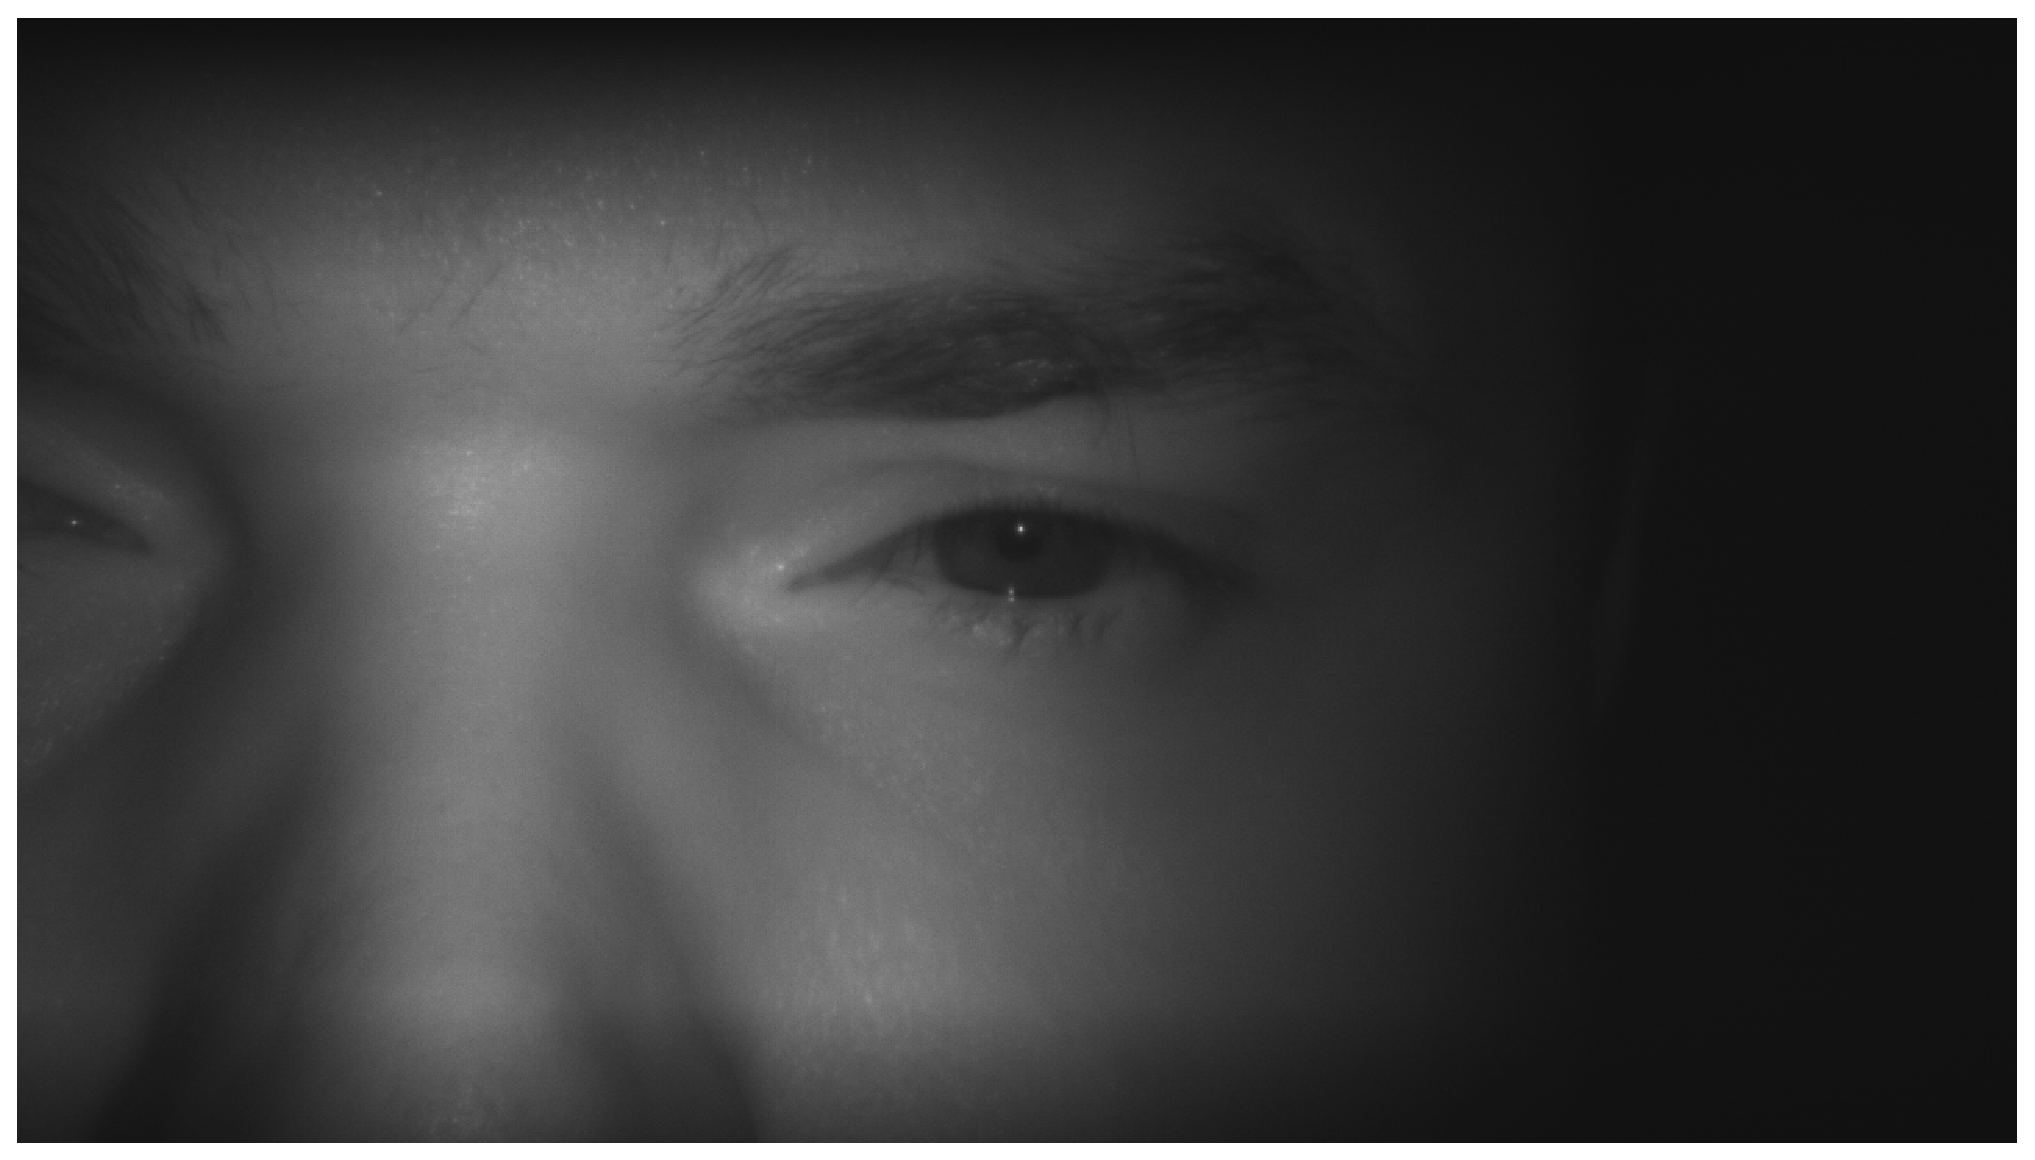
\includegraphics[width=0.95\columnwidth]{pictures/mobile_db_example_30.eps}
		\label{fig:mobile_db_example_18}
	\end{subfigure}%
	\begin{subfigure}{.475\textwidth}
		\centering
		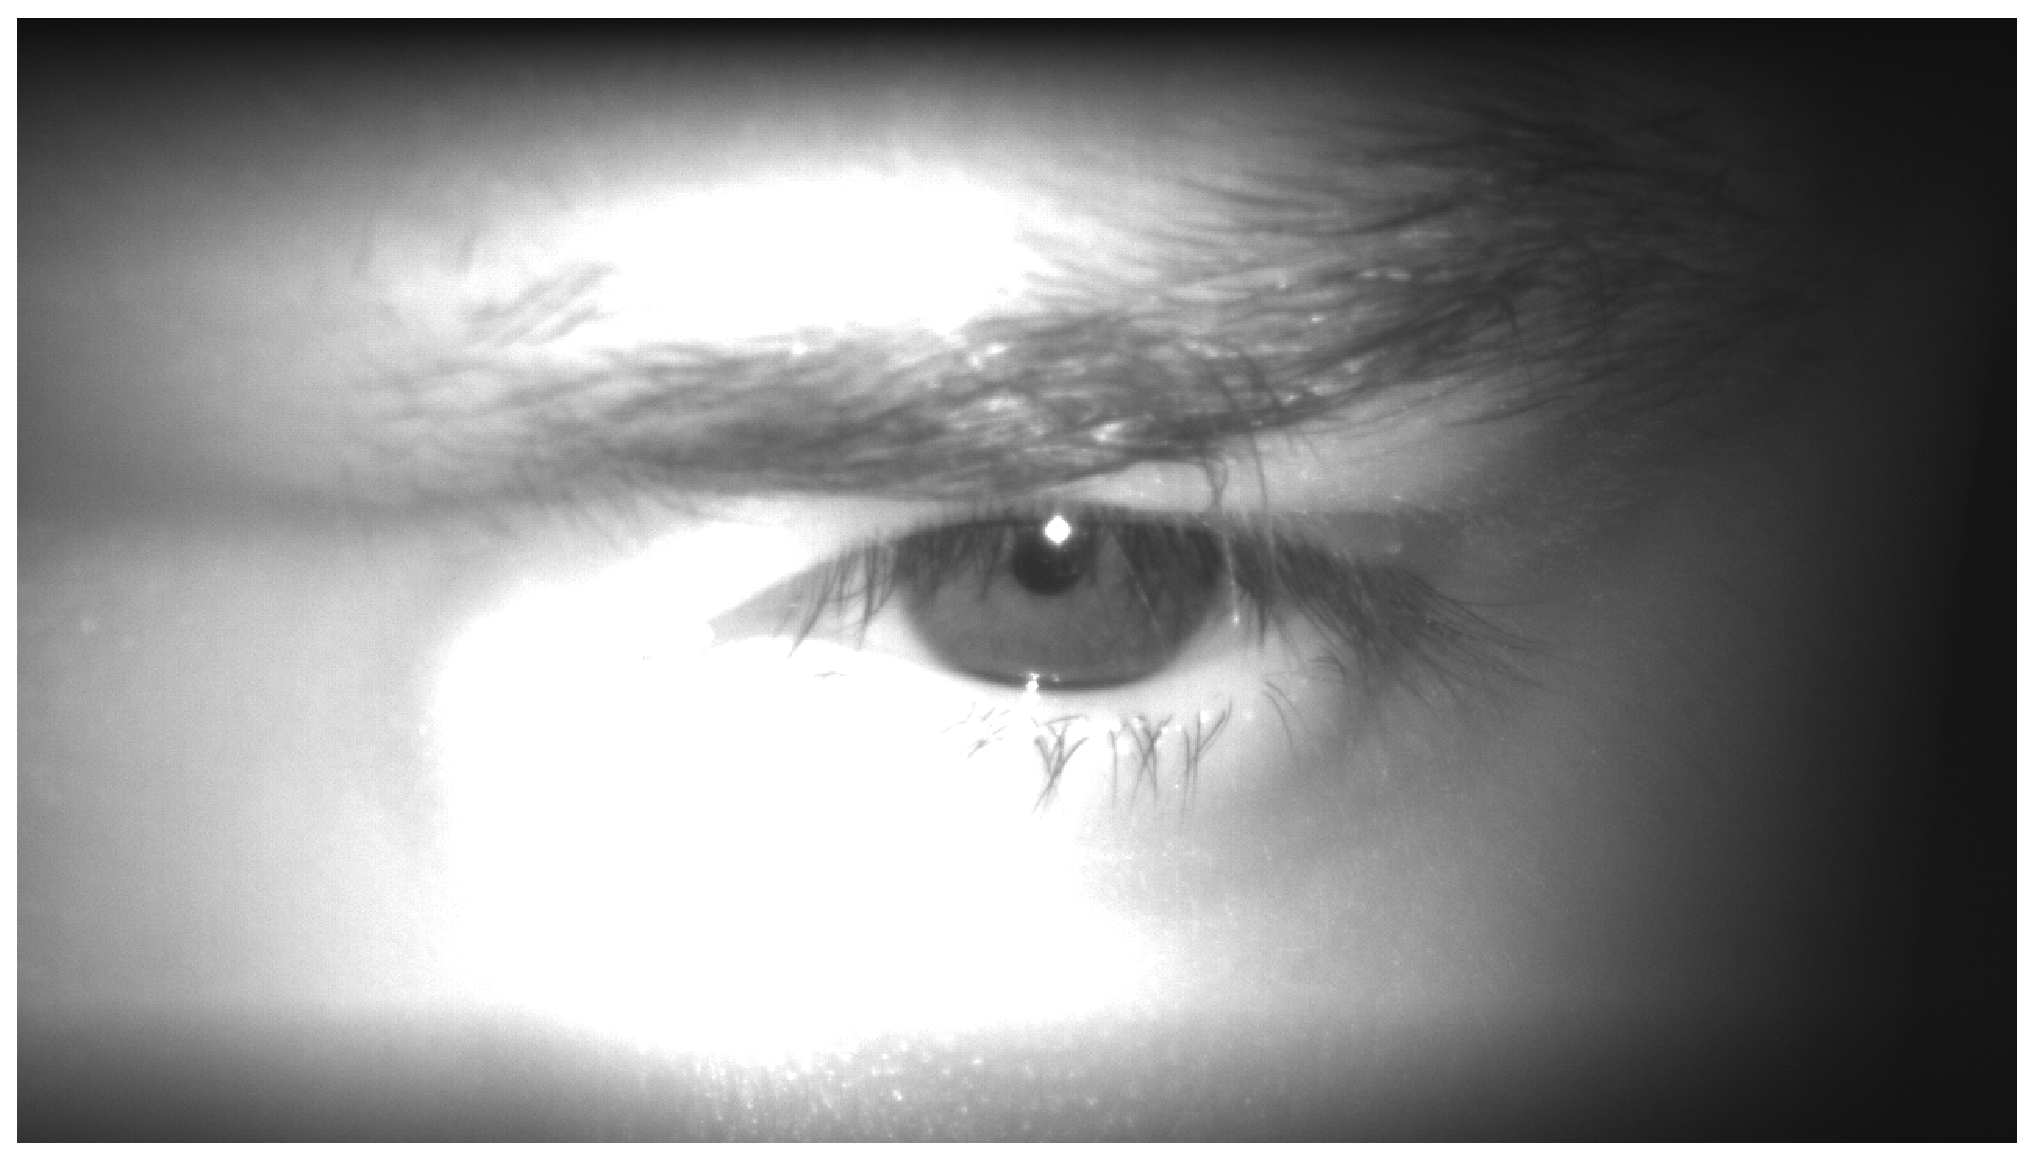
\includegraphics[width=0.95\columnwidth]{pictures/mobile_db_example_18.eps}
		\label{fig:mobile_db_example_30}
	\end{subfigure}%
	\caption{Примеры изображений, полученных на разных расстояниях от лица до устройства: 18 и 30 (см) слева и справа соответственно}
	\label{fig:mobiel_db_examples}
\end{figure}

Примеры изображений, снятых камерой, представлены на Рис.~\ref{fig:mobiel_db_examples}. Изображения взяты из одной и той же видеопоследовательности, но соответствуют разным расстояниям (18 и 30 см). Все видеопоследовательности используются для моделирования попыток регистрации и верификации. Для обоих сценариев использовались одни и те же параметры алгоритма, поэтому значение $FTE$ равно значению $FTA$ (Таб.~\ref{tab:accuracy_results}).

{\bf Результаты по точности распознавания}

В соответствии с общепринятыми понятиями и определениями, подробно описанными, например, в~\cite{dunstone_biosystem}, а также стандартах ISO/IЕС 19795-1:2006, ISO/IEC 19794-6:2011 и ГОСТ Р ИСО/МЭК 19795-1-2007, для оценивания производительности системы распознавания были выбраны следующие (основные):

\begin{itemize}
	\setlength\itemsep{0.01em}
	\item[$\bullet$] FTE (failure to enroll) - количество транзакций регистрации, для которых не возможно завершить извлечение биометрического эталона;
	\item[$\bullet$] FTA (failure to acquire) - количество транзакций верификации, для которых не возможно завершить извлечение биометрического эталона;
	\item[$\bullet$] Степень схожести - численная мера близости двух биометрических эталонов;
	\item[$\bullet$] FNMR (false non-match rate) - вероятность ложного несовпадения;
	\item[$\bullet$] FMR (false match rate) - вероятность ложного совпадения;
	\item[$\bullet$] EER (equal error rate) - равный уровень ошибок, коэффициент, при котором FNMR=FMR;
	\item[$\bullet$] Enrollment template - биометрический шаблон, полученный в режиме регистрации, содержащий один или несколько биометрических эталонов;
	\item[$\bullet$] Probe template - биометрический шаблон, полученный в режиме верификации, содержащий один или несколько биометрических эталонов;
\end{itemize}

Полученные результаты по точности распознавания предложенного алгоритма представлены в таблице~\ref{tab:accuracy_results}. Данные значения были получены с использованием системы автоматического тестирования и базы данных, описанной в таблице~\ref{tab:dataset_spec}.

{\bf Процедура тестирования} состояла из нескольких этапов:
\begin{enumerate}
	\setlength\itemsep{0.01em}
	\item Формирование биометрических эталонов из всех видеопоследовательностей в режиме регистрации;
	\item Формирование биометрических эталонов из всех видеопоследовательностей в режиме верификации;
	\item Формирование списка всех возможных пар сравнений шаблонов (enrollment-probe);
	\item Вычисление значений степени схожести для каждой из пар биометрических шаблонов;
	\item Вычисление показателей точности распознавания (Таб.~\ref{tab:accuracy_results});
\end{enumerate}

Оценка FTA и FTE производится по результатам выполнения шагов 1 и 2. Полученные значения (Таб.~\ref{tab:accuracy_results}) отражают возможность метода обрабатывать данные, полученные в сложных условиях.

Поскольку система аутентификации представляет собой бинарный классификатор, точность распознавания для нее оценивается с помощью ROC (receiver operating characteristic) кривой, отражающей зависимость между величинами FMR и FNMR~\cite{enc_biometrics}. Значения FMR и FNMR изменяются в зависимости от внутренних параметров системы распознавания, таких как порог принятия решения, с которым сравнивается полученное значение степени схожести биометрических эталонов, а также самих значений степени схожести. Более подробно о процедуре оценивания описано в работе~\cite{odinokikh_hprec_2018}.


\begin{table}[h]
	\begin{center}
		\small
		\begin{tabular}{|l|c|c|}
			\hline
			Значение	& Без очков   	& С очками\\
			\hline
			FTA/FTE		& 0.0685        & 0.07001 \\
			FMR			& $10^{-7}$     & $10^{-6}$ \\
			FNMR		& 0.01077       & 0.03912 \\
			EER			& 0.00128       & 0.00574 \\
			\hline
		\end{tabular}
	\end{center}
	\caption{Результаты по точности распознавания}
	\label{tab:accuracy_results}
\end{table}

{\bf Результаты по скорости распознавания}

Производительность метода оценивалась при помощи вышеупомянутого планшета, оснащенного процессором Qualcomm Snapdragon 800 (2.26 GHz, Quad-core). Измерения производились на одном ядре процессора. Медианное время выполнения составило 25 и 42 (мсек) для операций первого и второго блоков (\ref{subsec:algorithm_structure}, Рис.~\ref{fig:algorithm_structure}) соответственно.

\section{Выводы ко второй главе}

Рассмотрены основные трудности, связанные с биометрическим распознаванием человека по радужной оболочке глаза при помощи мобильного устройства. Предложены, протестированы и внедрены:

\begin{enumerate}
	\item новая многостадийная структура алгоритма для автоматического распознавания, построенная с использованием промежуточных блоков оценки качества изображения, позволяющая осуществлять распознавание человека при помощи устройства со значительно ограниченной вычислительной мощностью в режиме реального времени ($\approx15$ кадров/сек.), удовлетворяющая критериями ошибок: $FNMR\leq1\%$ при $FMR<10^{-7}$;
	\item алгоритм оценки качества, позволяющий:
	\begin{itemize}
		\item[$\bullet$] комплексно оценивать качество входящего изображения радужки на предмет его пригодности для извлечения признаков и формирования биометрического эталона;
		\item[$\bullet$] обеспечивать обратную связь с пользователем путем отображения подсказок, понятных пользователю, на экране устройства, на основании внутренних измеряемых показателей качества изображения;
		\item[$\bullet$] производить управление параметрами системы регистрации изображения с целью получения изображения радужки наилучшего качества;
		\item[$\bullet$] учитывать и использовать данные с иных доступных сенсоров, позволяющих получать дополнительную информацию об окружении.
	\end{itemize}
\end{enumerate}
